\documentclass[12pt, letterpaper]{article}

\usepackage[T1]{fontenc}
\usepackage[utf8]{inputenc}
\usepackage{babel}
\usepackage{mathptmx}
\usepackage[top=2cm,bottom=2cm,left=3cm,right=2cm,headheight=15pt]{geometry}
\usepackage{setspace}
\usepackage{ragged2e}
\usepackage{titlesec}
\usepackage{booktabs}
\usepackage{array}
\usepackage{longtable}
\usepackage{graphicx}
\usepackage{caption}
\usepackage{hyperref}
\usepackage{amsmath}
\usepackage{microtype}
\usepackage{parskip}
\usepackage{fancyhdr}

\setstretch{1.5}
\justifying

\titleformat{\section}[block]
  {\normalfont\large\bfseries\centering}
  {\Roman{section}.}{0.5em}{\MakeUppercase}

\titleformat{\subsection}[block]
  {\normalfont\normalsize\itshape}
  {\Alph{subsection}.}{0.5em}{}

\titleformat{\subsubsection}[runin]
  {\normalfont\normalsize\itshape}
  {\arabic{subsubsection})}{0.5em}{}[:]

\titlespacing*{\section}{0pt}{12pt}{6pt}
\titlespacing*{\subsection}{0pt}{10pt}{4pt}
\titlespacing*{\subsubsection}{1em}{8pt}{0.5em}

\renewcommand{\thetable}{\Roman{table}}
\captionsetup[table]{
  labelfont=bf,
  textfont=normalfont,
  labelsep=newline,
  justification=centering,
  position=top,
  name=TABLA
}

\renewcommand{\thefigure}{\arabic{figure}}
\captionsetup[figure]{
  labelfont=bf,
  textfont=normalfont,
  labelsep=period,
  justification=centering,
  position=bottom,
  name=Figura
}

\renewcommand{\contentsname}{\'Indice de Contenido}
\renewcommand{\listfigurename}{\'Indice de Figuras}
\renewcommand{\listtablename}{\'Indice de Tablas}
\renewcommand{\figurename}{Figura}
\renewcommand{\tablename}{TABLA}
\renewcommand{\refname}{Referencias}
\renewcommand{\abstractname}{Resumen}

\pagestyle{fancy}
\fancyhf{}
\renewcommand{\headrulewidth}{0.4pt}
\renewcommand{\footrulewidth}{0.4pt}
\fancyhead[L]{\small\textit{Sistema Omnicanal --- Gesti\'on de Mesas, \'Ordenes y Pagos}}
\fancyhead[R]{\small\textit{Trabajo Terminal}}
\fancyfoot[C]{\small\thepage}

\hypersetup{
  colorlinks=true,
  linkcolor=black,
  urlcolor=black,
  citecolor=black,
  pdftitle={Bouquet - Diccionario de Base de Datos},
  pdfauthor={},
}

\setlength{\LTpre}{0pt}
\setlength{\LTpost}{0pt}

\begin{document}

% ══════════════════════════════════════════════════════════════
% DICCIONARIO DE DATOS — BOUQUET OPS
% Sistema Omnicanal para Gestión de Mesas, Órdenes y Pagos
% ══════════════════════════════════════════════════════════════

\section{Diseño de Base de Datos}

\subsection{Convenciones del Modelo}

El modelo de datos de \textbf{Bouquet OPS} sigue las siguientes convenciones globales:

\begin{itemize}
  \item Todos los identificadores primarios son de tipo \texttt{text} y se generan como UUIDs v4 en la capa de aplicación.
  \item Los valores monetarios se almacenan como enteros en \textbf{centavos} (\texttt{int}) para evitar errores de precisión propios del tipo \texttt{float}. Por ejemplo, \$149.90 MXN se representa como \texttt{14990}.
  \item Las tasas porcentuales (impuestos, propinas) se almacenan en \textbf{basis points} (\texttt{int}), donde $100\,\text{bps} = 1\%$. Por ejemplo, IVA 16\% se representa como \texttt{1600}.
  \item Los campos \texttt{archivedAt} de tipo \texttt{timestamp nullable} implementan eliminación lógica (\textit{soft delete}). Un valor \texttt{NULL} indica que el registro está activo; un valor no nulo indica que fue archivado. Los registros no se eliminan físicamente para preservar la integridad histórica.
  \item Los campos \texttt{createdAt} y \texttt{updatedAt} están presentes en todas las tablas y son mantenidos automáticamente por la capa ORM.
  \item Las restricciones de unicidad compuesta (\texttt{UNIQUE}) y de verificación (\texttt{CHECK}) se documentan explícitamente en cada tabla.
\end{itemize}

\subsection{Dominios del Modelo}

El modelo se organiza en siete dominios lógicos:

\begin{enumerate}
  \item \textbf{Catálogos globales}: entidades de referencia compartidas por toda la plataforma.
  \item \textbf{Control de acceso (RBAC)}: roles, permisos y asignaciones contextuales.
  \item \textbf{Identidad}: usuarios del sistema y sus contextos de operación.
  \item \textbf{Organización}: jerarquía cadena → zona → restaurante.
  \item \textbf{Menú}: catálogo canónico por cadena e instancia vendible por restaurante.
  \item \textbf{Operación de mesa}: sesiones, mesas y comensales.
  \item \textbf{Transacciones}: órdenes, ítems, modificadores, pagos, reembolsos y descuentos.
\end{enumerate}

\begin{figure}[htbp]
  \centering
  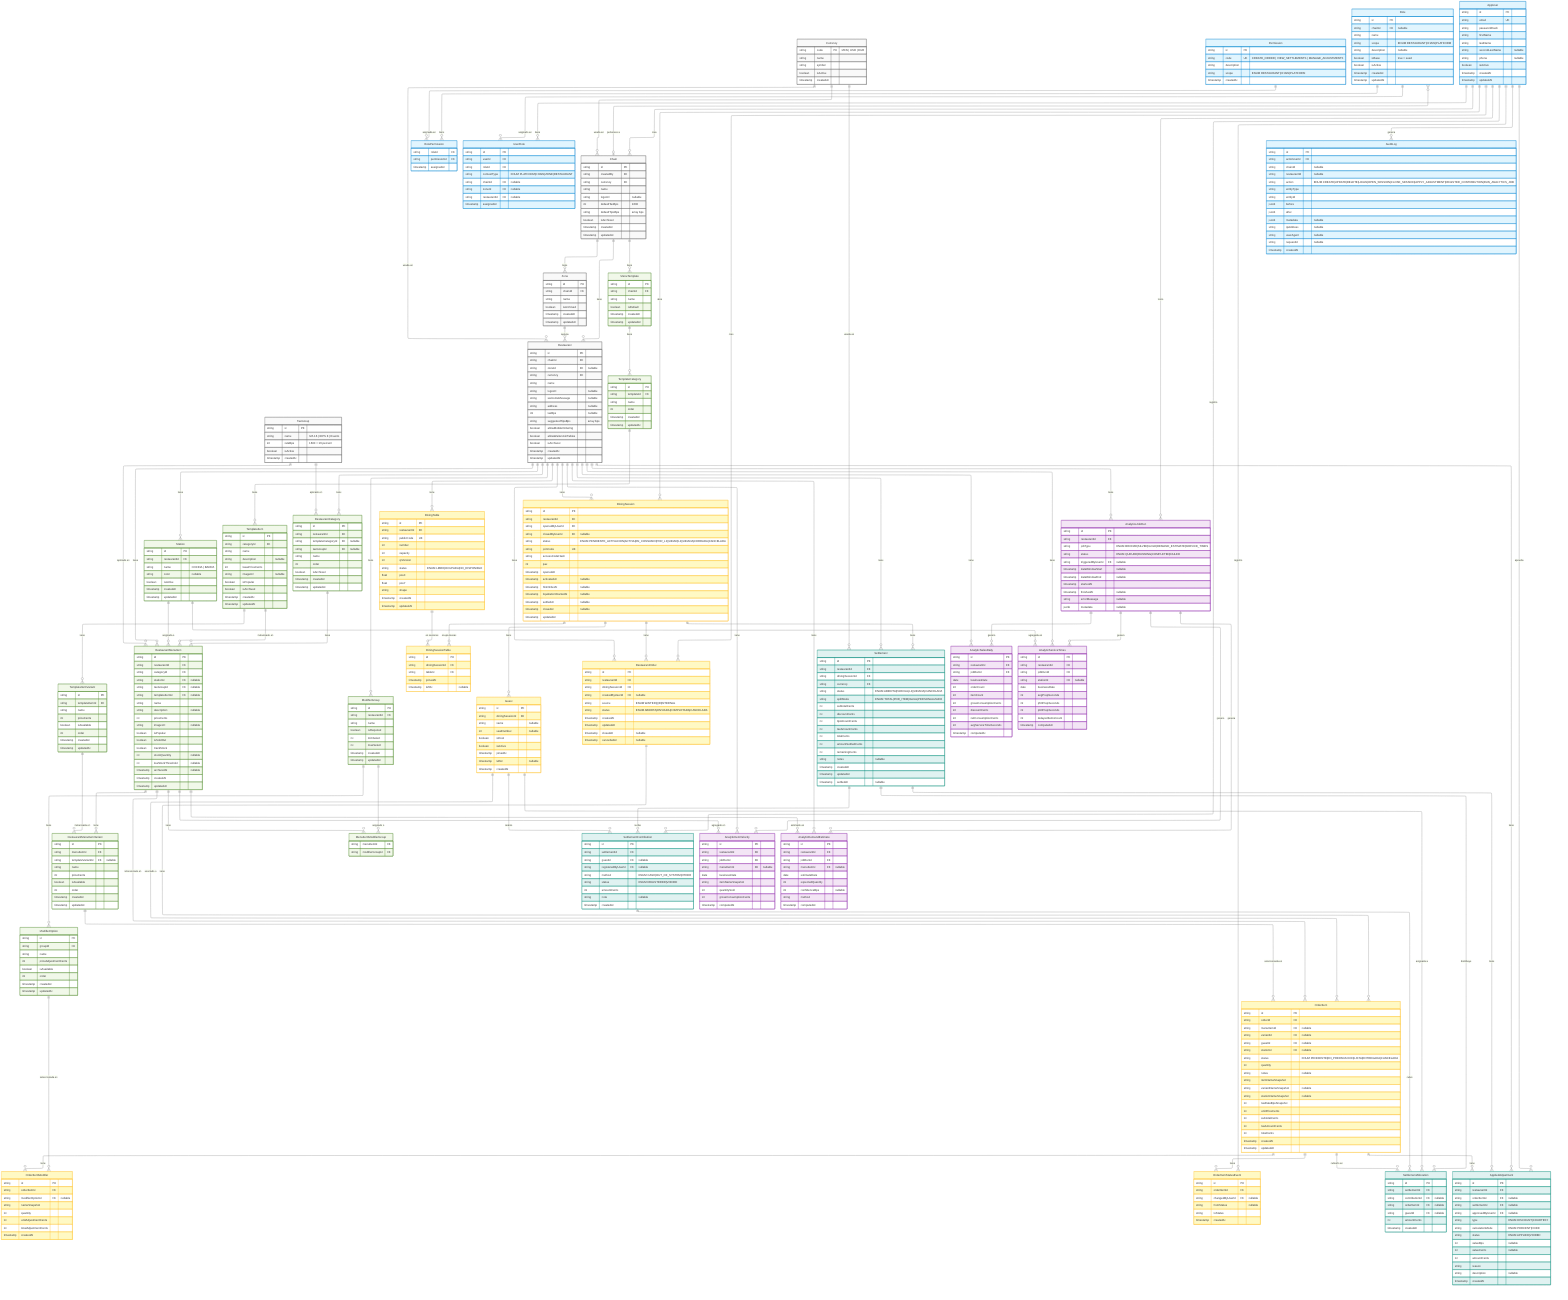
\includegraphics[width=\textwidth,height=0.9\textheight,keepaspectratio]{../_assets/erd/rendered/DB.pdf}
  \caption{Modelo de Entidad-Relación Global — Bouquet OPS}
  \label{fig:erd-global}
\end{figure}

\clearpage

% ══════════════════════════════════════════════════════════════
\subsection{Diccionario de Datos}
% ══════════════════════════════════════════════════════════════

% ── Macro para encabezado de tabla ──
% Uso: \tabladd{NombreTabla}{Descripción corta}
% Columnas: Campo | Tipo | Nulo | PK/FK | Descripción

\newcommand{\dictable}[2]{%
  \subsubsection{#1}
  #2
  \vspace{4pt}
  \begin{longtable}{|p{3.8cm}|p{2.2cm}|p{1cm}|p{1cm}|p{6.2cm}|}
  \hline
  \textbf{Campo} & \textbf{Tipo} & \textbf{Nulo} & \textbf{Clave} & \textbf{Descripción} \\
  \hline
  \endfirsthead
  \hline
  \textbf{Campo} & \textbf{Tipo} & \textbf{Nulo} & \textbf{Clave} & \textbf{Descripción} \\
  \hline
  \endhead
}

\newcommand{\dictableend}{%
  \hline
  \end{longtable}
}

% ── Fila estándar ──
\newcommand{\campo}[5]{\texttt{#1} & \texttt{#2} & #3 & #4 & #5 \\ \hline}

% Paquetes necesarios en el preámbulo del documento principal:
% \usepackage{longtable}
% \usepackage{booktabs}
% \usepackage{array}
% \usepackage{hyperref}

% ══════════════════════════════════════════════════════════════
% 1. CATÁLOGOS GLOBALES
% ══════════════════════════════════════════════════════════════

\subsubsection*{\textit{Dominio 1 — Catálogos Globales}}

\begin{center}
  \includegraphics[width=0.8\textwidth,height=0.4\textheight,keepaspectratio]{../_assets/erd/rendered/dominio-01-catalogos.pdf}
\end{center}

\dictable{Currency}{%
Catálogo de monedas soportadas por la plataforma. Permite que cadenas y restaurantes operen en diferentes divisas sin duplicar lógica de conversión. Nuevas monedas se agregan insertando un registro; no requiere cambios en el código.}
\campo{code}{text}{No}{PK}{Código ISO 4217 de la moneda (ej. \texttt{MXN}, \texttt{USD}, \texttt{EUR}). Sirve como clave primaria semántica.}
\campo{name}{text}{No}{—}{Nombre completo de la moneda (ej. \textit{Peso Mexicano}).}
\campo{symbol}{text}{No}{—}{Símbolo de representación visual (ej. \texttt{\$}, \texttt{€}).}
\campo{isActive}{boolean}{No}{—}{Indica si la moneda está disponible para su selección. Valor predeterminado: \texttt{true}.}
\campo{createdAt}{timestamp}{No}{—}{Fecha y hora de creación del registro.}
\dictableend

\newpage

\dictable{TaxGroup}{%
Catálogo de grupos de impuestos aplicables a categorías y productos. Permite modelar distintos regímenes fiscales (IVA, IEPS, tasa cero) sin acoplar la tasa directamente a cada producto.}
\campo{id}{text}{No}{PK}{Identificador único UUID.}
\campo{name}{text}{No}{—}{Nombre descriptivo del grupo (ej. \textit{IVA 16\%}, \textit{IEPS 8\%}, \textit{Exento}).}
\campo{rateBps}{int}{No}{—}{Tasa expresada en basis points. $1\,600 = 16\%$, $0 = $ exento.}
\campo{isActive}{boolean}{No}{—}{Indica si el grupo está disponible para asignación.}
\campo{createdAt}{timestamp}{No}{—}{Fecha y hora de creación del registro.}
\dictableend

% ══════════════════════════════════════════════════════════════
% 2. RBAC
% ══════════════════════════════════════════════════════════════

\newpage

\subsubsection*{\textit{Dominio 2 — Control de Acceso (RBAC)}}

\begin{center}
  \includegraphics[width=0.8\textwidth,height=0.4\textheight,keepaspectratio]{../_assets/erd/rendered/dominio-02-rbac.pdf}
\end{center}

\dictable{Permission}{%
Catálogo de permisos atómicos del sistema. Cada permiso representa una acción específica que puede realizarse en la plataforma (ej. \texttt{CREATE\_ORDER}, \texttt{VIEW\_PAYMENTS}). Los permisos se definen en tiempo de desarrollo y se asocian a roles mediante la tabla \texttt{RolePermission}.}
\campo{id}{text}{No}{PK}{Identificador único UUID.}
\campo{code}{text}{No}{UK}{Código único del permiso en formato \texttt{SCREAMING\_SNAKE\_CASE} (ej. \texttt{MANAGE\_MENU}).}
\campo{description}{text}{No}{—}{Descripción legible del permiso para interfaz administrativa.}
\campo{scope}{enum}{No}{—}{Nivel de aplicación del permiso: \texttt{PLATFORM}, \texttt{CHAIN} o \texttt{RESTAURANT}.}
\campo{createdAt}{timestamp}{No}{—}{Fecha y hora de creación.}
\dictableend

\newpage

\dictable{Role}{%
Roles del sistema de control de acceso basado en roles (RBAC). Un rol agrupa permisos y puede ser de plataforma (base, inmutable) o propio de una cadena (personalizable). Los roles base se insertan en el proceso de \textit{seed} inicial y no pueden eliminarse.}
\campo{id}{text}{No}{PK}{Identificador único UUID.}
\campo{chainId}{text}{Sí}{FK}{Referencia a \texttt{Chain}. \texttt{NULL} indica que es un rol base de plataforma, disponible para todas las cadenas.}
\campo{name}{text}{No}{—}{Nombre del rol (ej. \textit{ADMIN}, \textit{MESERO}, \textit{COCINA}).}
\campo{scope}{enum}{No}{—}{Nivel de operación del rol: \texttt{PLATFORM}, \texttt{CHAIN} o \texttt{RESTAURANT}.}
\campo{description}{text}{Sí}{—}{Descripción opcional del propósito del rol.}
\campo{isBase}{boolean}{No}{—}{Si es \texttt{true}, el rol fue creado en el \textit{seed} y no puede eliminarse.}
\campo{isActive}{boolean}{No}{—}{Indica si el rol está disponible para asignación.}
\campo{createdAt}{timestamp}{No}{—}{Fecha y hora de creación.}
\campo{updatedAt}{timestamp}{No}{—}{Fecha y hora de última modificación.}
\dictableend
\noindent\textbf{Restricción única:} \texttt{UNIQUE(chainId, name, scope)} — impide roles duplicados dentro del mismo contexto.


\dictable{RolePermission}{%
Tabla pivote que asocia roles con permisos. Define qué acciones puede realizar cada rol en la plataforma.}
\campo{roleId}{text}{No}{FK}{Referencia a \texttt{Role}.}
\campo{permissionId}{text}{No}{FK}{Referencia a \texttt{Permission}.}
\campo{assignedAt}{timestamp}{No}{—}{Fecha y hora en que se asignó el permiso al rol.}
\dictableend
\noindent\textbf{Clave primaria compuesta:} \texttt{(roleId, permissionId)}.


% ══════════════════════════════════════════════════════════════
% 3. IDENTIDAD
% ══════════════════════════════════════════════════════════════

\newpage
\subsubsection*{\textit{Dominio 3 — Identidad}}

\begin{center}
  \includegraphics[width=0.8\textwidth,height=0.4\textheight,keepaspectratio]{../_assets/erd/rendered/dominio-03-identidad.pdf}
\end{center}

\dictable{AppUser}{%
Tabla central de identidad del sistema. Unifica en un solo registro a todos los tipos de usuarios: superadministradores de plataforma, personal de cadena y personal de restaurante. La diferenciación de contexto y permisos se delega a la tabla \texttt{UserRole}.}
\campo{id}{text}{No}{PK}{Identificador único UUID.}
\campo{email}{text}{No}{UK}{Correo electrónico único en toda la plataforma. Utilizado como identificador de autenticación.}
\campo{passwordHash}{text}{No}{—}{Hash de la contraseña generado con \textit{bcrypt}. Nunca se almacena en texto plano.}
\campo{firstName}{text}{No}{—}{Nombre(s) del usuario.}
\campo{lastName}{text}{No}{—}{Apellido paterno.}
\campo{secondLastName}{text}{Sí}{—}{Apellido materno. Opcional para compatibilidad internacional.}
\campo{phone}{text}{Sí}{—}{Número de teléfono de contacto.}
\campo{isActive}{boolean}{No}{—}{Indica si la cuenta está habilitada para autenticación.}
\campo{isFirstLogin}{boolean}{No}{—}{Flag para forzar el cambio de contraseña en el primer inicio de sesión. Valor predeterminado: \texttt{true}.}
\campo{createdAt}{timestamp}{No}{—}{Fecha y hora de creación de la cuenta.}
\campo{updatedAt}{timestamp}{No}{—}{Fecha y hora de última modificación.}
\dictableend

\dictable{UserRole}{%
Tabla de asignación contextual de roles. Define en qué contexto (plataforma, cadena, zona o restaurante) opera cada usuario y con qué rol. Permite que un mismo usuario tenga roles distintos en diferentes contextos sin duplicar su identidad.}
\campo{id}{text}{No}{PK}{Identificador único UUID.}
\campo{userId}{text}{No}{FK}{Referencia a \texttt{AppUser}.}
\campo{roleId}{text}{No}{FK}{Referencia a \texttt{Role}.}
\campo{contextType}{enum}{No}{—}{Tipo de contexto: \texttt{PLATFORM}, \texttt{CHAIN}, \texttt{ZONE} o \texttt{RESTAURANT}.}
\campo{chainId}{text}{Sí}{FK}{Referencia a \texttt{Chain}. Poblado solo si \texttt{contextType = CHAIN}.}
\campo{zoneId}{text}{Sí}{FK}{Referencia a \texttt{Zone}. Poblado solo si \texttt{contextType = ZONE}.}
\campo{restaurantId}{text}{Sí}{FK}{Referencia a \texttt{Restaurant}. Poblado solo si \texttt{contextType = RESTAURANT}.}
\campo{assignedAt}{timestamp}{No}{—}{Fecha y hora en que se asignó el rol.}
\dictableend
\noindent\textbf{Restricción CHECK:} Exactamente uno de \texttt{chainId}, \texttt{zoneId} o \texttt{restaurantId} debe ser no nulo, según el valor de \texttt{contextType}. Para \texttt{PLATFORM}, los tres deben ser \texttt{NULL}.

\noindent\textbf{Restricción única:} \texttt{UNIQUE(userId, roleId, contextType, chainId, zoneId, restaurantId)}.


% ══════════════════════════════════════════════════════════════
% 4. ORGANIZACIÓN
% ══════════════════════════════════════════════════════════════

\subsubsection*{\textit{Dominio 4 — Organización}}

\begin{center}
  \includegraphics[width=0.9\textwidth,height=0.85\textheight,keepaspectratio]{../_assets/erd/rendered/dominio-04-organizacion.pdf}
\end{center}

\newpage

\dictable{Chain}{%
Representa una cadena de restaurantes. Es la entidad raíz de la jerarquía organizacional. Define configuraciones heredables por zonas y restaurantes, como moneda, tasa de impuesto predeterminada y sugerencias de propina.}
\campo{id}{text}{No}{PK}{Identificador único UUID.}
\campo{createdBy}{text}{No}{FK}{Referencia a \texttt{AppUser}. Usuario (superadministrador) que creó la cadena.}
\campo{currency}{text}{No}{FK}{Referencia a \texttt{Currency.code}. Moneda predeterminada de la cadena.}
\campo{name}{text}{No}{—}{Nombre comercial de la cadena.}
\campo{logoUrl}{text}{Sí}{—}{URL de la imagen del logotipo almacenada en Supabase Storage.}
\campo{defaultTaxBps}{int}{No}{—}{Tasa de impuesto predeterminada en basis points. Heredada por restaurantes que no definan la propia.}
\campo{defaultTipsBps}{int[]}{Sí}{—}{Arreglo de enteros en basis points con las opciones de propina sugeridas (ej. \texttt{[1000, 1500, 2000]} para 10\%, 15\%, 20\%). Heredado por restaurantes que no definan el propio.}
\campo{isArchived}{boolean}{No}{—}{Eliminación lógica de la cadena.}
\campo{createdAt}{timestamp}{No}{—}{Fecha y hora de creación.}
\campo{updatedAt}{timestamp}{No}{—}{Fecha y hora de última modificación.}
\dictableend

\newpage

\dictable{Zone}{%
Agrupación geográfica u organizacional de restaurantes dentro de una cadena. Permite que administradores de zona supervisen un subconjunto de sucursales sin acceso a toda la cadena.}
\campo{id}{text}{No}{PK}{Identificador único UUID.}
\campo{chainId}{text}{No}{FK}{Referencia a \texttt{Chain}. Cadena a la que pertenece la zona.}
\campo{name}{text}{No}{—}{Nombre de la zona (ej. \textit{Norte}, \textit{CDMX Centro}).}
\campo{isArchived}{boolean}{No}{—}{Eliminación lógica de la zona.}
\campo{createdAt}{timestamp}{No}{—}{Fecha y hora de creación.}
\campo{updatedAt}{timestamp}{No}{—}{Fecha y hora de última modificación.}
\dictableend
\noindent\textbf{Restricción única:} \texttt{UNIQUE(chainId, name)}.


\dictable{Restaurant}{%
Representa una sucursal o unidad de negocio operacional. Pertenece directamente a una cadena y opcionalmente a una zona. Es la entidad central del dominio operacional: mesas, órdenes y pagos siempre pertenecen a un restaurante.}
\campo{id}{text}{No}{PK}{Identificador único UUID.}
\campo{chainId}{text}{No}{FK}{Referencia a \texttt{Chain}. Relación directa con la cadena propietaria.}
\campo{zoneId}{text}{Sí}{FK}{Referencia a \texttt{Zone}. Opcional; permite restaurantes sin zona asignada.}
\campo{currency}{text}{No}{FK}{Referencia a \texttt{Currency.code}.}
\campo{name}{text}{No}{—}{Nombre de la sucursal.}
\campo{logoUrl}{text}{Sí}{—}{URL del logotipo propio de la sucursal.}
\campo{welcomeMessage}{text}{Sí}{—}{Mensaje de bienvenida mostrado en la interfaz QR del comensal.}
\campo{address}{text}{Sí}{—}{Dirección física, obtenida mediante autocompletado con Nominatim (OpenStreetMap).}
\campo{taxBps}{int}{Sí}{—}{Tasa de impuesto local en basis points. Si es \texttt{NULL}, hereda \texttt{Chain.defaultTaxBps}.}
\campo{suggestedTipsBps}{int[]}{Sí}{—}{Arreglo de opciones de propina en basis points. Si es \texttt{NULL}, hereda \texttt{Chain.defaultTipsBps}.}
\campo{allowMobileOrdering}{boolean}{No}{—}{Habilita la captura de órdenes desde QR por parte del comensal.}
\campo{allowWaiterJoinTables}{boolean}{No}{—}{Permite que los meseros unan mesas en grupos.}
\campo{isArchived}{boolean}{No}{—}{Eliminación lógica de la sucursal.}
\campo{createdAt}{timestamp}{No}{—}{Fecha y hora de creación.}
\campo{updatedAt}{timestamp}{No}{—}{Fecha y hora de última modificación.}
\dictableend

\newpage

\dictable{AuditLog}{%
Registro de auditoría de acciones realizadas por usuarios del sistema. Almacena un \textit{snapshot} del estado anterior y posterior de cada entidad modificada, junto con metadatos del contexto de la solicitud. Es inmutable: los registros nunca se modifican ni eliminan.}
\campo{id}{text}{No}{PK}{Identificador único UUID.}
\campo{actorUserId}{text}{No}{FK}{Referencia a \texttt{AppUser}. Usuario que realizó la acción.}
\campo{chainId}{text}{Sí}{—}{Identificador de la cadena en cuyo contexto ocurrió la acción.}
\campo{restaurantId}{text}{Sí}{—}{Identificador del restaurante en cuyo contexto ocurrió la acción.}
\campo{action}{enum}{No}{—}{Tipo de acción: \texttt{CREATE}, \texttt{UPDATE}, \texttt{ARCHIVE} o \texttt{DELETE}.}
\campo{entityType}{text}{No}{—}{Nombre de la entidad afectada (ej. \textit{Chain}, \textit{RestaurantMenuItem}).}
\campo{entityId}{text}{No}{—}{Identificador del registro afectado.}
\campo{before}{jsonb}{Sí}{—}{\textit{Snapshot} del estado anterior al cambio. \texttt{NULL} en operaciones \texttt{CREATE}.}
\campo{after}{jsonb}{Sí}{—}{\textit{Snapshot} del estado posterior al cambio. \texttt{NULL} en operaciones \texttt{DELETE}.}
\campo{metadata}{jsonb}{Sí}{—}{Información adicional del contexto (ej. parámetros de la solicitud).}
\campo{ipAddress}{text}{Sí}{—}{Dirección IP del cliente que originó la solicitud.}
\campo{userAgent}{text}{Sí}{—}{Agente de usuario del cliente HTTP.}
\campo{requestId}{text}{Sí}{—}{Identificador único de la solicitud HTTP para correlación de logs.}
\campo{createdAt}{timestamp}{No}{—}{Fecha y hora del evento. Inmutable.}
\dictableend

% ══════════════════════════════════════════════════════════════
% 5. MENÚ
% ══════════════════════════════════════════════════════════════

\subsubsection*{\textit{Dominio 5 — Menú}}

\begin{center}
  \includegraphics[width=\textwidth,height=0.85\textheight,keepaspectratio]{../_assets/erd/rendered/dominio-05-menu.pdf}
\end{center}

\newpage

\noindent El dominio de menú se divide en dos subcapas:

\begin{itemize}
  \item \textbf{Catálogo canónico (cadena):} \texttt{MenuTemplate}, \texttt{TemplateCategory}, \texttt{TemplateItem}, \texttt{TemplateItemVariant}. Funcionan como plantillas centralizadas. \textbf{No son entidades transaccionales}; los restaurantes no venden desde el template directamente.
  \item \textbf{Instancia local (restaurante):} \texttt{RestaurantCategory}, \texttt{RestaurantMenuItem}, \texttt{RestaurantMenuItemVariant}. Representan el menú vendible en cada sucursal. Pueden originarse desde un template (vía \texttt{templateItemId}) o crearse localmente.
\end{itemize}

\dictable{MenuTemplate}{%
Plantilla de menú centralizada definida a nivel de cadena. Permite estandarizar el catálogo de productos entre sucursales. Un restaurante puede basarse en un template para poblar su menú local, manteniendo trazabilidad al origen.}
\campo{id}{text}{No}{PK}{Identificador único UUID.}
\campo{chainId}{text}{No}{FK}{Referencia a \texttt{Chain}.}
\campo{name}{text}{No}{—}{Nombre del template (ej. \textit{Menú Estándar 2026}).}
\campo{isDefault}{boolean}{No}{—}{Indica si es el template predeterminado de la cadena.}
\campo{createdAt}{timestamp}{No}{—}{Fecha y hora de creación.}
\campo{updatedAt}{timestamp}{No}{—}{Fecha y hora de última modificación.}
\dictableend
\noindent\textbf{Restricción única:} \texttt{UNIQUE(chainId, name)}.


\dictable{TemplateCategory}{%
Categoría de productos dentro de un template de menú (ej. \textit{Entradas}, \textit{Bebidas}, \textit{Postres}).}
\campo{id}{text}{No}{PK}{Identificador único UUID.}
\campo{templateId}{text}{No}{FK}{Referencia a \texttt{MenuTemplate}.}
\campo{name}{text}{No}{—}{Nombre de la categoría.}
\campo{order}{int}{No}{—}{Posición de visualización dentro del template.}
\campo{createdAt}{timestamp}{No}{—}{Fecha y hora de creación.}
\campo{updatedAt}{timestamp}{No}{—}{Fecha y hora de última modificación.}
\dictableend

\dictable{TemplateItem}{%
Producto base definido en un template de menú. Establece el precio de referencia y atributos generales del producto. No se vende directamente; se instancia en \texttt{RestaurantMenuItem}.}
\campo{id}{text}{No}{PK}{Identificador único UUID.}
\campo{categoryId}{text}{No}{FK}{Referencia a \texttt{TemplateCategory}.}
\campo{name}{text}{No}{—}{Nombre del producto.}
\campo{description}{text}{Sí}{—}{Descripción del producto.}
\campo{basePriceCents}{int}{No}{—}{Precio base de referencia en centavos. Puede sobreescribirse en la instancia local.}
\campo{imageUrl}{text}{Sí}{—}{URL de imagen referencial.}
\campo{isPopular}{boolean}{No}{—}{Marca el producto como popular para destacarlo visualmente.}
\campo{isArchived}{boolean}{No}{—}{Eliminación lógica.}
\campo{createdAt}{timestamp}{No}{—}{Fecha y hora de creación.}
\campo{updatedAt}{timestamp}{No}{—}{Fecha y hora de última modificación.}
\dictableend

\dictable{TemplateItemVariant}{%
Variante de un producto en el template (ej. \textit{Chico}, \textit{Mediano}, \textit{Grande}). Define el precio y nombre de cada opción a nivel de plantilla.}
\campo{id}{text}{No}{PK}{Identificador único UUID.}
\campo{templateItemId}{text}{No}{FK}{Referencia a \texttt{TemplateItem}.}
\campo{name}{text}{No}{—}{Nombre de la variante.}
\campo{priceCents}{int}{No}{—}{Precio de esta variante en centavos.}
\campo{isAvailable}{boolean}{No}{—}{Indica si la variante está disponible.}
\campo{order}{int}{No}{—}{Posición de visualización.}
\campo{createdAt}{timestamp}{No}{—}{Fecha y hora de creación.}
\campo{updatedAt}{timestamp}{No}{—}{Fecha y hora de última modificación.}
\dictableend

\dictable{Station}{%
Estación de preparación dentro de un restaurante (ej. \textit{Cocina}, \textit{Barra}, \textit{Sushi}). Cada restaurante define sus propias estaciones. Los productos se asignan a una estación para que el KDS (\textit{Kitchen Display System}) enrute correctamente las comandas.}
\campo{id}{text}{No}{PK}{Identificador único UUID.}
\campo{restaurantId}{text}{No}{FK}{Referencia a \texttt{Restaurant}.}
\campo{name}{text}{No}{—}{Nombre de la estación.}
\campo{color}{text}{Sí}{—}{Color en formato hexadecimal para identificación visual en el KDS.}
\campo{isActive}{boolean}{No}{—}{Indica si la estación está operativa.}
\campo{createdAt}{timestamp}{No}{—}{Fecha y hora de creación.}
\campo{updatedAt}{timestamp}{No}{—}{Fecha y hora de última modificación.}
\dictableend
\noindent\textbf{Restricción única:} \texttt{UNIQUE(restaurantId, name)}.


\dictable{RestaurantCategory}{%
Categoría de productos del menú local de un restaurante. Puede tener un grupo de impuestos asociado que aplica a todos sus productos, salvo que un producto lo sobreescriba individualmente.}
\campo{id}{text}{No}{PK}{Identificador único UUID.}
\campo{restaurantId}{text}{No}{FK}{Referencia a \texttt{Restaurant}.}
\campo{taxGroupId}{text}{Sí}{FK}{Referencia a \texttt{TaxGroup}. Impuesto predeterminado para productos de esta categoría.}
\campo{name}{text}{No}{—}{Nombre de la categoría.}
\campo{order}{int}{No}{—}{Posición de visualización en el menú.}
\campo{isArchived}{boolean}{No}{—}{Eliminación lógica.}
\campo{createdAt}{timestamp}{No}{—}{Fecha y hora de creación.}
\campo{updatedAt}{timestamp}{No}{—}{Fecha y hora de última modificación.}
\dictableend
\noindent\textbf{Restricción única:} \texttt{UNIQUE(restaurantId, name)}.


\dictable{RestaurantMenuItem}{%
Producto vendible en un restaurante específico. Es la única entidad desde la cual se generan ítems de orden. Puede originarse desde un \texttt{TemplateItem} (vía \texttt{templateItemId}) o crearse de forma completamente local. El precio, disponibilidad, estación y stock son atributos propios de la instancia local y no afectan al template de origen.}
\campo{id}{text}{No}{PK}{Identificador único UUID.}
\campo{restaurantId}{text}{No}{FK}{Referencia a \texttt{Restaurant}.}
\campo{categoryId}{text}{No}{FK}{Referencia a \texttt{RestaurantCategory}.}
\campo{stationId}{text}{Sí}{FK}{Referencia a \texttt{Station}. \texttt{NULL} si el producto no requiere preparación en KDS (ej. bebida embotellada).}
\campo{taxGroupId}{text}{Sí}{FK}{Referencia a \texttt{TaxGroup}. Sobreescribe el impuesto de la categoría si se especifica.}
\campo{templateItemId}{text}{Sí}{FK}{Referencia a \texttt{TemplateItem}. \texttt{NULL} si es producto local sin origen en template.}
\campo{name}{text}{No}{—}{Nombre del producto tal como se muestra al comensal.}
\campo{description}{text}{Sí}{—}{Descripción del producto.}
\campo{priceCents}{int}{No}{—}{Precio de venta en centavos en este restaurante.}
\campo{imageUrl}{text}{Sí}{—}{URL de imagen del producto.}
\campo{isPopular}{boolean}{No}{—}{Marca el producto como popular.}
\campo{isSoldOut}{boolean}{No}{—}{Indica agotamiento manual del producto.}
\campo{trackStock}{boolean}{No}{—}{Si es \texttt{true}, el sistema descuenta \texttt{stockQuantity} con cada venta.}
\campo{stockQuantity}{int}{Sí}{—}{Unidades disponibles. Solo relevante si \texttt{trackStock = true}.}
\campo{lowStockThreshold}{int}{Sí}{—}{Umbral mínimo para alerta de stock bajo.}
\campo{archivedAt}{timestamp}{Sí}{—}{Fecha de archivado lógico. \texttt{NULL} indica producto activo. Los productos no se eliminan físicamente para conservar integridad histórica.}
\campo{createdAt}{timestamp}{No}{—}{Fecha y hora de creación.}
\campo{updatedAt}{timestamp}{No}{—}{Fecha y hora de última modificación.}
\dictableend

\dictable{RestaurantMenuItemVariant}{%
Variante vendible de un producto en el restaurante (ej. \textit{Chico}, \textit{Mediano}, \textit{Grande}). Si el producto se originó desde un template, puede mantener referencia a la variante original.}
\campo{id}{text}{No}{PK}{Identificador único UUID.}
\campo{menuItemId}{text}{No}{FK}{Referencia a \texttt{RestaurantMenuItem}.}
\campo{templateVariantId}{text}{Sí}{FK}{Referencia a \texttt{TemplateItemVariant}. \texttt{NULL} si la variante es local.}
\campo{name}{text}{No}{—}{Nombre de la variante.}
\campo{priceCents}{int}{No}{—}{Precio de la variante en centavos.}
\campo{isAvailable}{boolean}{No}{—}{Indica si la variante puede seleccionarse.}
\campo{order}{int}{No}{—}{Posición de visualización.}
\campo{createdAt}{timestamp}{No}{—}{Fecha y hora de creación.}
\campo{updatedAt}{timestamp}{No}{—}{Fecha y hora de última modificación.}
\dictableend

\dictable{ModifierGroup}{%
Grupo de modificadores aplicables a uno o más productos (ej. \textit{Extras}, \textit{Término de cocción}, \textit{Sin ingrediente}). Define si la selección es obligatoria y cuántas opciones pueden elegirse.}
\campo{id}{text}{No}{PK}{Identificador único UUID.}
\campo{restaurantId}{text}{No}{FK}{Referencia a \texttt{Restaurant}.}
\campo{name}{text}{No}{—}{Nombre del grupo de modificadores.}
\campo{isRequired}{boolean}{No}{—}{Si es \texttt{true}, el comensal debe seleccionar al menos una opción.}
\campo{minSelect}{int}{No}{—}{Número mínimo de opciones seleccionables. \texttt{0} indica opcional.}
\campo{maxSelect}{int}{No}{—}{Número máximo de opciones seleccionables. \texttt{1} implica selección única (radio).}
\campo{createdAt}{timestamp}{No}{—}{Fecha y hora de creación.}
\campo{updatedAt}{timestamp}{No}{—}{Fecha y hora de última modificación.}
\dictableend

\dictable{ModifierOption}{%
Opción individual dentro de un grupo de modificadores (ej. \textit{Extra queso}, \textit{Sin cebolla}, \textit{Bien cocido}). Puede tener un ajuste de precio adicional.}
\campo{id}{text}{No}{PK}{Identificador único UUID.}
\campo{groupId}{text}{No}{FK}{Referencia a \texttt{ModifierGroup}.}
\campo{name}{text}{No}{—}{Nombre de la opción.}
\campo{priceAdjustmentCents}{int}{No}{—}{Ajuste de precio en centavos. \texttt{0} si no tiene costo adicional.}
\campo{isAvailable}{boolean}{No}{—}{Indica si la opción está disponible para selección.}
\campo{order}{int}{No}{—}{Posición de visualización dentro del grupo.}
\campo{createdAt}{timestamp}{No}{—}{Fecha y hora de creación.}
\campo{updatedAt}{timestamp}{No}{—}{Fecha y hora de última modificación.}
\dictableend
\noindent\textbf{Restricción única:} \texttt{UNIQUE(groupId, name)}.


\dictable{MenuItemModifierGroup}{%
Tabla pivote que asocia grupos de modificadores con productos del menú local. Define qué grupos de opciones están disponibles al ordenar un producto específico.}
\campo{menuItemId}{text}{No}{FK}{Referencia a \texttt{RestaurantMenuItem}.}
\campo{modifierGroupId}{text}{No}{FK}{Referencia a \texttt{ModifierGroup}.}
\dictableend

\noindent\textbf{Clave primaria compuesta:} \texttt{(menuItemId, modifierGroupId)}.

% ══════════════════════════════════════════════════════════════
% 6. OPERACIÓN DE MESA
% ══════════════════════════════════════════════════════════════

\newpage

\subsubsection*{\textit{Dominio 6 — Operación de Mesa}}

\begin{center}
  \includegraphics[width=0.8\textwidth,height=0.5\textheight,keepaspectratio]{../_assets/erd/rendered/dominio-06-mesa.pdf}
\end{center}

\dictable{DiningTable}{%
Representa una mesa física dentro de un restaurante. Contiene su posición en el plano del salón para la vista de mapa, y un token de QR rotativo para el acceso de comensales. El campo \texttt{status} funciona como caché operacional: su valor se deriva del estado de las sesiones activas y debe mantenerse sincronizado mediante lógica transaccional en la capa de aplicación.}
\campo{id}{text}{No}{PK}{Identificador único UUID.}
\campo{restaurantId}{text}{No}{FK}{Referencia a \texttt{Restaurant}.}
\campo{number}{int}{No}{—}{Número identificador de la mesa dentro del restaurante.}
\campo{capacity}{int}{No}{—}{Capacidad máxima de comensales.}
\campo{qrTokenHash}{text}{No}{—}{Hash del token público del código QR. El token en texto claro viaja en el QR; la base de datos guarda únicamente su hash para comparación segura.}
\campo{qrVersion}{int}{No}{—}{Versión del QR. Se incrementa al regenerar el código, invalidando versiones anteriores.}
\campo{status}{enum}{No}{—}{Caché del estado operativo: \texttt{DISPONIBLE}, \texttt{OCUPADA} o \texttt{RESERVADA}. Derivado de \texttt{DiningSessionTable} y sincronizado transaccionalmente.}
\campo{posX}{float}{No}{—}{Posición horizontal en el plano del salón (en píxeles o unidades relativas).}
\campo{posY}{float}{No}{—}{Posición vertical en el plano del salón.}
\campo{shape}{text}{No}{—}{Forma visual de la mesa: \texttt{rect} o \texttt{circle}.}
\campo{createdAt}{timestamp}{No}{—}{Fecha y hora de creación.}
\campo{updatedAt}{timestamp}{No}{—}{Fecha y hora de última modificación.}
\dictableend
\noindent\textbf{Restricción única:} \texttt{UNIQUE(restaurantId, number)}.

\newpage

\dictable{DiningSession}{%
Representa una visita activa de comensales al restaurante. Es la entidad contenedora de órdenes y pagos. Una sesión puede ocupar una o varias mesas (mediante \texttt{DiningSessionTable}) y contener múltiples comensales individuales (mediante \texttt{Guest}).}
\campo{id}{text}{No}{PK}{Identificador único UUID.}
\campo{restaurantId}{text}{No}{FK}{Referencia a \texttt{Restaurant}.}
\campo{openedByUserId}{text}{No}{FK}{Referencia a \texttt{AppUser}. Personal que abrió la sesión.}
\campo{closedByUserId}{text}{Sí}{FK}{Referencia a \texttt{AppUser}. Personal que cerró la sesión. \texttt{NULL} si la sesión está abierta.}
\campo{status}{enum}{No}{—}{Estado de la sesión: \texttt{OPEN}, \texttt{CLOSED} o \texttt{CANCELLED}.}
\campo{pax}{int}{No}{—}{Número total de comensales en la sesión.}
\campo{openedAt}{timestamp}{No}{—}{Fecha y hora de apertura.}
\campo{closedAt}{timestamp}{Sí}{—}{Fecha y hora de cierre. \texttt{NULL} si la sesión está activa.}
\campo{updatedAt}{timestamp}{No}{—}{Fecha y hora de última modificación.}
\dictableend

\newpage

\dictable{DiningSessionTable}{%
Tabla de relación entre sesiones y mesas. Permite que una sesión ocupe múltiples mesas simultáneamente y registra el historial de unión y separación de mesas durante una visita.}
\campo{id}{text}{No}{PK}{Identificador único UUID.}
\campo{diningSessionId}{text}{No}{FK}{Referencia a \texttt{DiningSession}.}
\campo{tableId}{text}{No}{FK}{Referencia a \texttt{DiningTable}.}
\campo{joinedAt}{timestamp}{No}{—}{Fecha y hora en que la mesa se unió a la sesión.}
\campo{leftAt}{timestamp}{Sí}{—}{Fecha y hora en que la mesa se separó. \texttt{NULL} si la mesa sigue activa en la sesión.}
\dictableend

\dictable{Guest}{%
Representa a un comensal individual dentro de una sesión. Permite dividir cuentas por persona y asociar ítems de orden a comensales específicos. El nombre es opcional para sesiones de autoservicio vía QR.}
\campo{id}{text}{No}{PK}{Identificador único UUID.}
\campo{diningSessionId}{text}{No}{FK}{Referencia a \texttt{DiningSession}.}
\campo{name}{text}{Sí}{—}{Nombre del comensal. Opcional.}
\campo{seatNumber}{int}{Sí}{—}{Número de asiento o lugar en la mesa. Opcional.}
\campo{createdAt}{timestamp}{No}{—}{Fecha y hora de registro.}
\dictableend

% ══════════════════════════════════════════════════════════════
% 7. TRANSACCIONES
% ══════════════════════════════════════════════════════════════
\newpage
\subsubsection*{\textit{Dominio 7 — Transacciones}}

\begin{center}
  \includegraphics[width=\textwidth,height=0.6\textheight,keepaspectratio]{../_assets/erd/rendered/dominio-07-transacciones.pdf}
\end{center}

\dictable{RestaurantOrder}{%
Comanda enviada por un mesero, comensal vía QR o punto de venta. Agrupa los ítems ordenados en un momento determinado dentro de una sesión. Una sesión puede contener múltiples órdenes (ej. entrada, plato fuerte y postre en tiempos distintos).}
\campo{id}{text}{No}{PK}{Identificador único UUID.}
\campo{restaurantId}{text}{No}{FK}{Referencia a \texttt{Restaurant}.}
\campo{diningSessionId}{text}{No}{FK}{Referencia a \texttt{DiningSession}.}
\campo{createdByUserId}{text}{Sí}{FK}{Referencia a \texttt{AppUser}. \texttt{NULL} si la orden fue generada por el comensal vía QR.}
\campo{source}{enum}{No}{—}{Canal de origen: \texttt{WAITER}, \texttt{QR} o \texttt{POS}.}
\campo{status}{enum}{No}{—}{Estado de la orden: \texttt{OPEN}, \texttt{SENT}, \texttt{PARTIALLY\_READY}, \texttt{READY}, \texttt{CLOSED} o \texttt{CANCELLED}.}
\campo{createdAt}{timestamp}{No}{—}{Fecha y hora de creación.}
\campo{updatedAt}{timestamp}{No}{—}{Fecha y hora de última modificación.}
\campo{closedAt}{timestamp}{Sí}{—}{Fecha y hora de cierre. Útil para reportes de tiempo de servicio.}
\campo{cancelledAt}{timestamp}{Sí}{—}{Fecha y hora de cancelación, si aplica.}
\dictableend

\newpage

\dictable{OrderItem}{%
Ítem individual dentro de una orden. Almacena un \textit{snapshot} completo del producto al momento de ordenar (nombre, precio, variante, estación) para garantizar la integridad histórica independientemente de modificaciones posteriores al catálogo.}
\campo{id}{text}{No}{PK}{Identificador único UUID.}
\campo{orderId}{text}{No}{FK}{Referencia a \texttt{RestaurantOrder}.}
\campo{menuItemId}{text}{Sí}{FK}{Referencia a \texttt{RestaurantMenuItem}. Nullable para preservar el historial si el producto es archivado.}
\campo{variantId}{text}{Sí}{FK}{Referencia a \texttt{RestaurantMenuItemVariant}. \texttt{NULL} si no se seleccionó variante.}
\campo{guestId}{text}{Sí}{FK}{Referencia a \texttt{Guest}. Permite asociar el ítem a un comensal específico para división de cuenta.}
\campo{stationId}{text}{Sí}{FK}{Referencia a \texttt{Station}. \textit{Snapshot} de la estación al momento de ordenar.}
\campo{status}{enum}{No}{—}{Estado del ítem en cocina: \texttt{NEW}, \texttt{SENT}, \texttt{PREPARING}, \texttt{READY}, \texttt{SERVED} o \texttt{CANCELLED}.}
\campo{quantity}{int}{No}{—}{Cantidad ordenada.}
\campo{notes}{text}{Sí}{—}{Instrucciones libres del comensal (ej. \textit{sin cebolla}, \textit{extra cocido}).}
\campo{itemNameSnapshot}{text}{No}{—}{\textit{Snapshot} del nombre del producto al momento de ordenar.}
\campo{variantNameSnapshot}{text}{Sí}{—}{\textit{Snapshot} del nombre de la variante seleccionada.}
\campo{unitPriceCents}{int}{No}{—}{\textit{Snapshot} del precio unitario en centavos al momento de ordenar.}
\campo{subtotalCents}{int}{No}{—}{Subtotal en centavos (\texttt{unitPriceCents × quantity}).}
\campo{taxAmountCents}{int}{No}{—}{Monto de impuesto calculado en centavos.}
\campo{totalCents}{int}{No}{—}{Total del ítem en centavos (\texttt{subtotalCents + taxAmountCents}).}
\campo{createdAt}{timestamp}{No}{—}{Fecha y hora de creación.}
\campo{updatedAt}{timestamp}{No}{—}{Fecha y hora de última modificación.}
\dictableend

\dictable{OrderItemModifier}{%
Modificador seleccionado para un ítem de orden (ej. \textit{Extra queso}, \textit{Sin cebolla}). Guarda un \textit{snapshot} del nombre y precio del modificador al momento de ordenar.}
\campo{id}{text}{No}{PK}{Identificador único UUID.}
\campo{orderItemId}{text}{No}{FK}{Referencia a \texttt{OrderItem}.}
\campo{modifierOptionId}{text}{Sí}{FK}{Referencia a \texttt{ModifierOption}. Nullable para preservar historial si la opción es eliminada.}
\campo{nameSnapshot}{text}{No}{—}{\textit{Snapshot} del nombre del modificador al momento de ordenar.}
\campo{quantity}{int}{No}{—}{Cantidad del modificador aplicada (ej. doble extra queso = 2).}
\campo{priceAdjustmentCents}{int}{No}{—}{\textit{Snapshot} del ajuste de precio en centavos al momento de ordenar.}
\campo{createdAt}{timestamp}{No}{—}{Fecha y hora de creación.}
\dictableend

\newpage

\dictable{OrderItemStatusEvent}{%
Historial de transiciones de estado de un ítem de orden. Permite al KDS rastrear el flujo completo de preparación de cada producto, desde la recepción hasta la entrega.}
\campo{id}{text}{No}{PK}{Identificador único UUID.}
\campo{orderItemId}{text}{No}{FK}{Referencia a \texttt{OrderItem}.}
\campo{changedByUserId}{text}{Sí}{FK}{Referencia a \texttt{AppUser}. \texttt{NULL} si la transición fue automática.}
\campo{fromStatus}{enum}{No}{—}{Estado anterior del ítem.}
\campo{toStatus}{enum}{No}{—}{Estado nuevo del ítem.}
\campo{createdAt}{timestamp}{No}{—}{Fecha y hora de la transición. Inmutable.}
\dictableend

\dictable{Payment}{%
Registro de un pago realizado dentro de una sesión. Un pago puede cubrir la cuenta completa o una parte de ella, dependiendo del modo de división seleccionado. Se liga a la sesión, no directamente a una orden, para soportar pagos que cubren múltiples órdenes.}
\campo{id}{text}{No}{PK}{Identificador único UUID.}
\campo{restaurantId}{text}{No}{FK}{Referencia a \texttt{Restaurant}.}
\campo{diningSessionId}{text}{No}{FK}{Referencia a \texttt{DiningSession}.}
\campo{currency}{text}{No}{FK}{Referencia a \texttt{Currency.code}.}
\campo{processedByUserId}{text}{Sí}{FK}{Referencia a \texttt{AppUser}. Personal que procesó el pago. \texttt{NULL} si fue autoservicio.}
\campo{status}{enum}{No}{—}{Estado del pago: \texttt{PENDING}, \texttt{PROCESSING}, \texttt{COMPLETED}, \texttt{FAILED}, \texttt{CANCELLED} o \texttt{REFUNDED}.}
\campo{method}{enum}{No}{—}{Método de pago: \texttt{CARD}, \texttt{CASH} o \texttt{TRANSFER}.}
\campo{splitMode}{enum}{No}{—}{Modo de división: \texttt{FULL} (cuenta completa), \texttt{BY\_ITEM} (por producto) o \texttt{EQUAL} (partes iguales).}
\campo{splitCount}{int}{No}{—}{Número total de partes en que se divide la cuenta.}
\campo{paxPaid}{int}{No}{—}{Número de personas que cubre este pago.}
\campo{subtotalCents}{int}{No}{—}{Subtotal en centavos antes de propina e impuestos.}
\campo{tipAmountCents}{int}{No}{—}{Monto de propina en centavos.}
\campo{taxAmountCents}{int}{No}{—}{Monto de impuesto en centavos.}
\campo{totalCents}{int}{No}{—}{Total a pagar en centavos.}
\campo{amountPaidCents}{int}{No}{—}{Monto efectivamente recibido en centavos.}
\campo{notes}{text}{Sí}{—}{Notas opcionales del pago.}
\campo{providerReference}{text}{Sí}{—}{Identificador de transacción del proveedor externo (Stripe, Mercado Pago, etc.).}
\campo{createdAt}{timestamp}{No}{—}{Fecha y hora de creación.}
\campo{updatedAt}{timestamp}{No}{—}{Fecha y hora de última modificación.}
\campo{paidAt}{timestamp}{Sí}{—}{Fecha y hora de confirmación del pago.}
\dictableend

\newpage

\dictable{PaymentAllocation}{%
Detalle de asignación de un pago a ítems específicos de la orden o comensales. Se utiliza cuando el \texttt{splitMode} es \texttt{BY\_ITEM} o \texttt{EQUAL}. Para pagos con \texttt{splitMode = FULL}, no se requieren registros de asignación.}
\campo{id}{text}{No}{PK}{Identificador único UUID.}
\campo{paymentId}{text}{No}{FK}{Referencia a \texttt{Payment}.}
\campo{orderItemId}{text}{Sí}{FK}{Referencia a \texttt{OrderItem}. Obligatorio si \texttt{splitMode = BY\_ITEM}.}
\campo{guestId}{text}{Sí}{FK}{Referencia a \texttt{Guest}. Indica qué comensal realizó este pago parcial.}
\campo{amountCents}{int}{No}{—}{Monto asignado en centavos.}
\campo{createdAt}{timestamp}{No}{—}{Fecha y hora de creación.}
\dictableend
\noindent\textbf{Restricción CHECK:} Al menos uno de \texttt{orderItemId} o \texttt{guestId} debe ser no nulo.


\dictable{Refund}{%
Registro de un reembolso asociado a un pago. Permite trazabilidad de devoluciones parciales o totales, incluyendo referencia al identificador del proveedor de pagos cuando aplica.}
\campo{id}{text}{No}{PK}{Identificador único UUID.}
\campo{paymentId}{text}{No}{FK}{Referencia a \texttt{Payment}.}
\campo{createdByUserId}{text}{No}{FK}{Referencia a \texttt{AppUser}. Personal que autorizó el reembolso.}
\campo{amountCents}{int}{No}{—}{Monto reembolsado en centavos.}
\campo{reason}{text}{No}{—}{Motivo del reembolso.}
\campo{status}{enum}{No}{—}{Estado del reembolso: \texttt{PENDING}, \texttt{COMPLETED} o \texttt{FAILED}.}
\campo{providerRefundId}{text}{Sí}{—}{Identificador del reembolso en el proveedor externo de pagos.}
\campo{createdAt}{timestamp}{No}{—}{Fecha y hora de creación.}
\campo{updatedAt}{timestamp}{No}{—}{Fecha y hora de última modificación.}
\dictableend

\dictable{AppliedDiscount}{%
Registro de un descuento aplicado a un ítem de orden o a un pago. Permite trazabilidad de cortesías, descuentos de gerente y promociones. Un descuento se aplica a un ítem \textbf{o} a un pago, nunca a ambos simultáneamente.}
\campo{id}{text}{No}{PK}{Identificador único UUID.}
\campo{restaurantId}{text}{No}{FK}{Referencia a \texttt{Restaurant}.}
\campo{orderItemId}{text}{Sí}{FK}{Referencia a \texttt{OrderItem}. Exclusivo con \texttt{paymentId}.}
\campo{paymentId}{text}{Sí}{FK}{Referencia a \texttt{Payment}. Exclusivo con \texttt{orderItemId}.}
\campo{approvedByUserId}{text}{Sí}{FK}{Referencia a \texttt{AppUser}. Personal que autorizó el descuento. \texttt{NULL} si es automático.}
\campo{type}{enum}{No}{—}{Tipo de descuento: \texttt{PERCENT} o \texttt{FIXED}.}
\campo{valueBps}{int}{Sí}{—}{Porcentaje en basis points. Poblado solo si \texttt{type = PERCENT}.}
\campo{valueCents}{int}{Sí}{—}{Valor fijo en centavos. Poblado solo si \texttt{type = FIXED}.}
\campo{amountCents}{int}{No}{—}{Monto final descontado en centavos, calculado al momento de aplicación.}
\campo{reason}{text}{No}{—}{Motivo obligatorio del descuento.}
\campo{description}{text}{Sí}{—}{Descripción adicional opcional.}
\campo{createdAt}{timestamp}{No}{—}{Fecha y hora de aplicación. Inmutable.}
\dictableend
\noindent\textbf{Restricción CHECK (XOR):} Exactamente uno de \texttt{orderItemId} o \texttt{paymentId} debe ser no nulo.

\noindent\textbf{Restricción CHECK (tipo):} Si \texttt{type = PERCENT}, \texttt{valueBps} debe ser no nulo y \texttt{valueCents} debe ser nulo. Si \texttt{type = FIXED}, \texttt{valueCents} debe ser no nulo y \texttt{valueBps} debe ser nulo.


% ══════════════════════════════════════════════════════════════
\subsection{Descripción de Relaciones}
% ══════════════════════════════════════════════════════════════

\subsubsection{Jerarquía Organizacional}

\texttt{Chain} es la entidad raíz. Puede contener múltiples \texttt{Zone}s y múltiples \texttt{Restaurant}s. La relación \texttt{Restaurant.zoneId} es opcional: un restaurante siempre pertenece a una cadena (\texttt{chainId} obligatorio), pero puede o no pertenecer a una zona. Esto permite operar sucursales individuales sin necesidad de crear zonas artificiales.

\subsubsection{Jerarquía de Menú}

El catálogo canónico (\texttt{MenuTemplate → TemplateCategory → TemplateItem → TemplateItemVariant}) vive a nivel de cadena y sirve como plantilla centralizada. Al instanciar un producto en un restaurante, se crea un \texttt{RestaurantMenuItem} que puede referenciar al \texttt{TemplateItem} de origen (\texttt{templateItemId}) o ser completamente independiente. \textbf{El restaurante vende únicamente desde \texttt{RestaurantMenuItem}}; los templates no participan en el flujo transaccional.

\subsubsection{Operación de Mesa}

Una \texttt{DiningSession} agrupa toda la actividad de una visita: mesas ocupadas (\texttt{DiningSessionTable}), comensales (\texttt{Guest}), órdenes (\texttt{RestaurantOrder}) y pagos (\texttt{Payment}). Una sesión puede ocupar varias mesas simultáneamente, y el historial de qué mesas estuvieron activas se preserva en \texttt{DiningSessionTable.leftAt}.

\subsubsection{Flujo de Orden}

Cada \texttt{RestaurantOrder} pertenece a una \texttt{DiningSession}. Una sesión puede tener múltiples órdenes (distintos momentos del servicio). Cada \texttt{OrderItem} registra un snapshot completo del producto al momento de ordenar, garantizando integridad histórica. Los modificadores seleccionados se registran en \texttt{OrderItemModifier} con sus propios snapshots. Las transiciones de estado de cada ítem se registran en \texttt{OrderItemStatusEvent} para alimentar el KDS.

\subsubsection{Flujo de Pago}

Un \texttt{Payment} se liga a una \texttt{DiningSession} para poder cubrir múltiples órdenes. El modo de división (\texttt{splitMode}) determina si se requieren \texttt{PaymentAllocation}s: \texttt{FULL} no las requiere; \texttt{BY\_ITEM} requiere \texttt{orderItemId} en cada allocation; \texttt{EQUAL} distribuye por comensal (\texttt{guestId}). Los reembolsos se registran en \texttt{Refund} con referencia al pago original. Los descuentos se registran en \texttt{AppliedDiscount} con restricción XOR entre ítem y pago.

% ══════════════════════════════════════════════════════════════
\subsection{Reglas de Negocio del Modelo}
% ══════════════════════════════════════════════════════════════

\begin{enumerate}

  \item \textbf{Herencia de configuración.} Si \texttt{Restaurant.taxBps} es \texttt{NULL}, se hereda \texttt{Chain.defaultTaxBps}. Si \texttt{Restaurant.suggestedTipsBps} es \texttt{NULL}, se hereda \texttt{Chain.defaultTipsBps}. La lógica de herencia se aplica en la capa de aplicación al calcular totales.

  \item \textbf{Eliminación lógica.} Los registros de productos (\texttt{RestaurantMenuItem}), categorías y otras entidades de catálogo no se eliminan físicamente. Se marca \texttt{archivedAt} con la fecha de archivado. Esto preserva la integridad de los \texttt{OrderItem} históricos que referencian productos ya descatalogados.

  \item \textbf{Snapshots en órdenes.} Al crear un \texttt{OrderItem}, se deben copiar el nombre del producto, nombre de variante, precio unitario, monto de impuesto y estación desde el catálogo vigente. Los snapshots son inmutables: cambios posteriores al catálogo no afectan órdenes existentes.

  \item \textbf{Estado de mesa como caché.} \texttt{DiningTable.status} es un campo derivado. Su valor correcto se determina consultando \texttt{DiningSessionTable}: si existe un registro con \texttt{leftAt IS NULL} asociado a una \texttt{DiningSession} con \texttt{status = OPEN}, la mesa está \texttt{OCUPADA}. El campo se actualiza transaccionalmente al abrir o cerrar sesiones para optimizar consultas del mapa de mesas.

  \item \textbf{Unicidad de email entre usuarios.} \texttt{AppUser.email} tiene restricción \texttt{UNIQUE} global. Un mismo correo electrónico no puede estar registrado dos veces en el sistema, independientemente del rol o contexto.

  \item \textbf{Contexto de rol consistente.} En \texttt{UserRole}, exactamente uno de \texttt{chainId}, \texttt{zoneId} o \texttt{restaurantId} debe ser no nulo, según \texttt{contextType}. Para \texttt{contextType = PLATFORM}, los tres deben ser \texttt{NULL}. Esta regla se enforza mediante restricción \texttt{CHECK} en la base de datos.

  \item \textbf{Roles base inmutables.} Los roles con \texttt{isBase = true} no pueden eliminarse ni modificarse desde la interfaz administrativa. Son parte del \textit{seed} inicial del sistema.

  \item \textbf{Descuento exclusivo.} Un \texttt{AppliedDiscount} se aplica a un ítem de orden \textbf{o} a un pago completo, nunca a ambos. Se enforza con restricción \texttt{CHECK} XOR.

  \item \textbf{Tipo de descuento consistente.} Si \texttt{AppliedDiscount.type = PERCENT}, \texttt{valueBps} debe ser no nulo y \texttt{valueCents} debe ser nulo. Si \texttt{type = FIXED}, la relación es inversa.

  \item \textbf{Allocation de pago.} Para \texttt{splitMode = FULL}, no se requieren registros en \texttt{PaymentAllocation}. Para \texttt{BY\_ITEM}, cada allocation debe tener \texttt{orderItemId} no nulo. Para \texttt{EQUAL}, la suma de allocations debe ser igual a \texttt{Payment.totalCents}.

  \item \textbf{Token QR seguro.} La base de datos almacena únicamente el hash del token QR (\texttt{qrTokenHash}). El token en texto claro viaja embebido en el código QR. Al recibir una solicitud, el sistema hashea el token recibido y lo compara con el almacenado. Al regenerar el QR, se incrementa \texttt{qrVersion} y se actualiza \texttt{qrTokenHash}, invalidando todos los QR previos de esa mesa.

  \item \textbf{Menú canónico vs. transaccional.} Los templates de menú (\texttt{MenuTemplate} y sus dependientes) no participan en el flujo transaccional. Las órdenes siempre referencian \texttt{RestaurantMenuItem}. El \texttt{templateItemId} en \texttt{RestaurantMenuItem} es únicamente informativo para trazabilidad de origen.

  \item \textbf{Valores monetarios enteros.} Todos los cálculos monetarios se realizan en centavos (\texttt{int}) para evitar errores de precisión de punto flotante. La conversión a formato de display (ej. \$149.90) se realiza en la capa de presentación dividiendo entre 100.

\end{enumerate}

\end{document}